\documentclass[tikz, border=6pt]{standalone}
\usepackage{amsmath,amssymb,bm}
\usepackage{newtxtext,newtxmath}   % Times-like text and math
\usepackage{tikz}
\usetikzlibrary{shapes.geometric, arrows.meta, positioning, calc, fit, backgrounds, shapes.symbols}
\definecolor{cExpert}{HTML}{8C8C8C}
\definecolor{cPolicy}{HTML}{E07B1A}
\definecolor{cCal}{HTML}{3B7DD1}
\definecolor{cBlend}{HTML}{4A8FD6}
\definecolor{cTrain}{HTML}{9DC08B}
\definecolor{cCollect}{HTML}{F5C08A}
\definecolor{cData}{HTML}{E9E9E9}
\definecolor{cBase}{HTML}{F1E4B8}
\definecolor{cOpen}{HTML}{B08BC9}
\definecolor{cOpenLine}{HTML}{7A4F96}
\definecolor{cLab1}{HTML}{F2A541}
\definecolor{cLab2}{HTML}{E0821F}
\definecolor{cLab3}{HTML}{C95D08}
\begin{document}
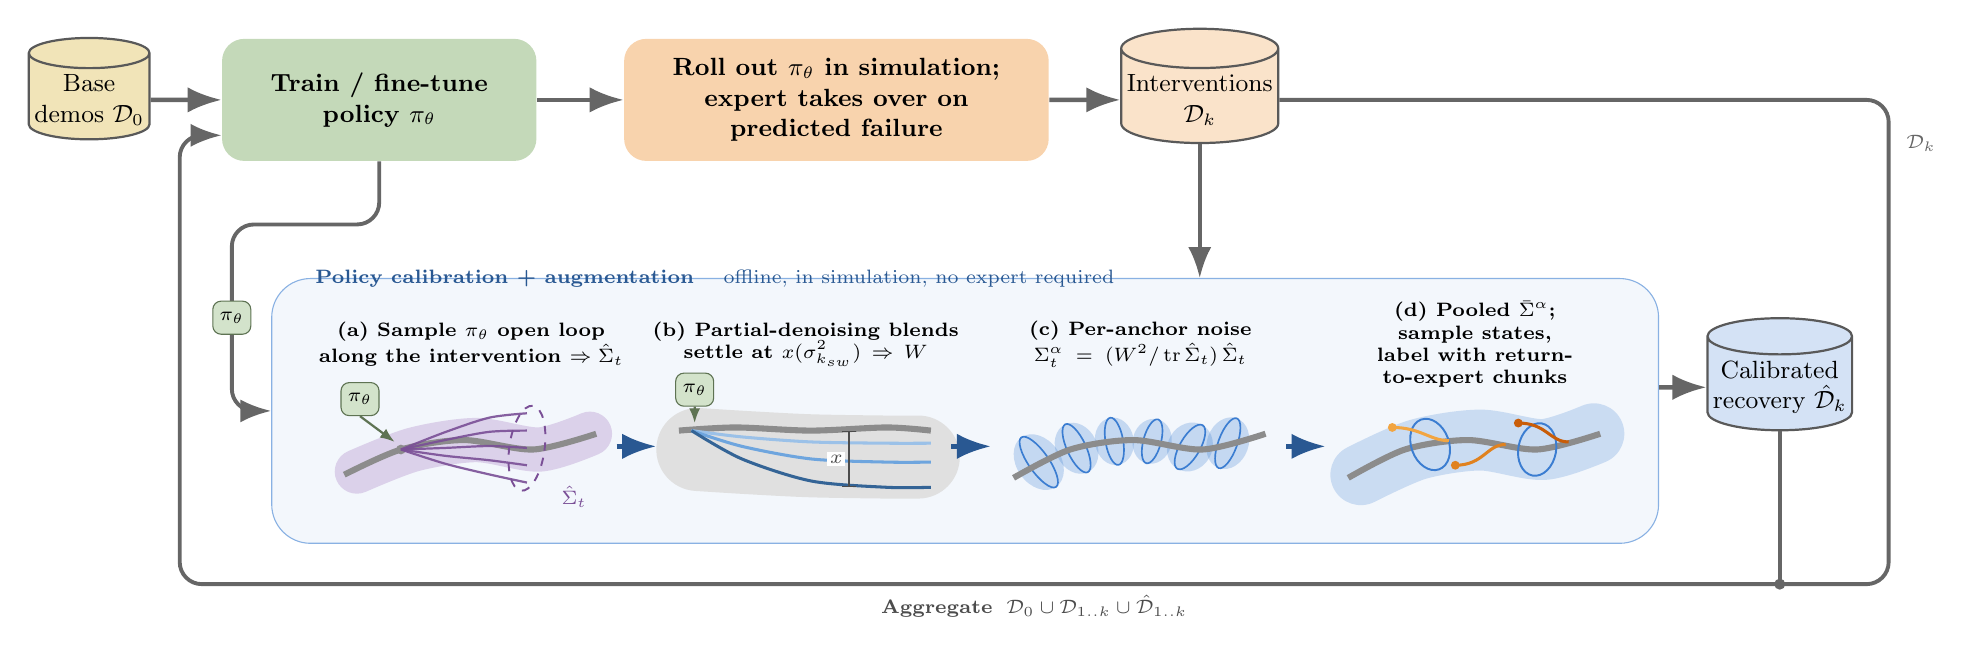
\begin{tikzpicture}[
  >=Stealth, font=\rmfamily,
  block/.style={rectangle, rounded corners=8pt, minimum height=1.55cm, align=center, font=\rmfamily\bfseries\small, inner sep=7pt, text width=3.5cm},
  data/.style={cylinder, shape border rotate=90, aspect=0.25, draw=black!65, line width=0.8pt, fill=cData, minimum width=1.5cm, minimum height=1.1cm, align=center, font=\rmfamily\small, inner sep=2pt},
  flow/.style={-{Latex[scale=1.2]}, line width=1.6pt, draw=black!60},
  loop/.style={-{Latex[scale=1.2]}, line width=1.4pt, draw=black!60, rounded corners=8pt},
  lab/.style={font=\rmfamily\scriptsize, align=center},
  paneltitle/.style={font=\rmfamily\bfseries\scriptsize, align=center, text width=3.9cm},
  formula/.style={font=\scriptsize, align=center, text width=3.9cm},
  region/.style={rounded corners=14pt, inner sep=8pt},
  chip/.style={rectangle, rounded corners=3pt, draw=cTrain!60!black, fill=cTrain!45, font=\rmfamily\bfseries\scriptsize, inner sep=2.5pt, minimum height=0.42cm}
]
% ================= Row 1: the DAgger loop =================
\node[data, fill=cBase] (D0) at (0,0) {Base\\demos $\mathcal{D}_0$};
\node[block, fill=cTrain!60, right=0.9cm of D0] (train) {Train / fine-tune\\policy $\pi_\theta$};
\node[block, fill=cCollect!70, right=1.1cm of train, text width=4.9cm] (collect) {Roll out $\pi_\theta$ in simulation;\\expert takes over on\\predicted failure};
\node[data, fill=cCollect!45, right=0.9cm of collect] (Dk) {Interventions\\$\mathcal{D}_k$};
\draw[flow] (D0) -- (train);
\draw[flow] (train) -- (collect);
\draw[flow] (collect) -- (Dk);

% ================= Row 2: offline policy calibration + augmentation =================
\coordinate (rowy) at (0,-4.6);
% panel geometry: 4 panels, pitch PW; sketches drawn in an inner scope scaled 0.8
\def\PW{4.25}
% ---- panel (a): open-loop spread ----
\begin{scope}[shift={($(rowy)+(3.0,0)$)}]
  \node[paneltitle] at (1.85,1.5) {\textbf{(a)} Sample $\pi_\theta$ open loop\\along the intervention $\Rightarrow \hat\Sigma_t$};
  \begin{scope}[scale=0.8]
  \draw[cOpen, opacity=0.35, line width=16pt, line cap=round] plot[smooth] coordinates {(0.5,-0.15) (1.4,0.2) (2.4,0.35) (3.4,0.2) (4.2,0.45)};
  \draw[cExpert, line width=2.2pt] plot[smooth] coordinates {(0.3,-0.2) (1.2,0.2) (2.2,0.35) (3.3,0.2) (4.3,0.45)};
  \fill[cExpert] (1.2,0.2) circle (2.2pt);
  \node[chip] (chipA) at (0.55,1.0) {$\pi_\theta$}; \draw[-{Latex[scale=0.8]}, cTrain!60!black, line width=0.8pt] (chipA.south) -- (1.1,0.32);
  \foreach \dy in {-0.55,-0.3,-0.05,0.2,0.45}{
    \draw[cOpenLine, line width=0.8pt, opacity=0.9] plot[smooth] coordinates {(1.2,0.2) (1.9,0.25+0.5*\dy) (2.6,0.3+0.9*\dy) (3.2,0.28+1.1*\dy)};}
  \draw[cOpenLine, dashed, line width=0.7pt, rotate around={-8:(3.2,0.22)}] (3.2,0.22) ellipse (0.28 and 0.68);
  \node[lab, text=cOpenLine] at (3.95,-0.55) {$\hat\Sigma_t$};
  \end{scope}
\end{scope}
% ---- panel (b): closed-loop blends -> W ----
\begin{scope}[shift={($(rowy)+(3.0+\PW,0)$)}]
  \node[paneltitle] at (1.85,1.5) {\textbf{(b)} Partial-denoising blends\\settle at $x(\sigma^2_{k_{sw}}) \Rightarrow W$};
  \begin{scope}[scale=0.8]
  \draw[black!12, line width=30pt, line cap=round] plot[smooth] coordinates {(0.6,0.2) (1.4,0.15) (2.4,0.1) (3.6,0.08) (4.1,0.08)};
  \draw[cExpert, line width=2.2pt] plot[smooth] coordinates {(0.3,0.5) (1.2,0.55) (2.4,0.5) (3.6,0.55) (4.3,0.5)};
  \node[chip] (chipB) at (0.55,1.15) {$\pi_\theta$}; \draw[-{Latex[scale=0.8]}, cTrain!60!black, line width=0.8pt] (chipB.south) -- (0.55,0.62);
  \draw[cBlend!55!white, line width=1.1pt] plot[smooth] coordinates {(0.5,0.5) (1.3,0.4) (2.4,0.32) (3.6,0.3) (4.3,0.3)};
  \draw[cBlend!80!white, line width=1.1pt] plot[smooth] coordinates {(0.5,0.5) (1.3,0.25) (2.4,0.05) (3.6,0.0) (4.3,0.0)};
  \draw[cBlend!70!black, line width=1.1pt] plot[smooth] coordinates {(0.5,0.5) (1.3,0.05) (2.4,-0.3) (3.6,-0.4) (4.3,-0.4)};
  \draw[black!70, {Bar}-{Bar}, line width=0.6pt] (3.0,0.5) -- (3.0,-0.4) node[midway, left=1pt, font=\scriptsize, fill=white, inner sep=1pt] {$x$};
  \end{scope}
\end{scope}
% ---- panel (c): per-anchor calibrated noise ----
\begin{scope}[shift={($(rowy)+(3.0+2*\PW,0)$)}]
  \node[paneltitle] at (1.85,1.5) {\textbf{(c)} Per-anchor noise\\$\Sigma^{\alpha}_t = (W^2/\operatorname{tr}\hat\Sigma_t)\,\hat\Sigma_t$};
  \begin{scope}[scale=0.8]
  \foreach \x/\y/\ang/\ra/\rb in {0.7/0.0/35/0.16/0.48, 1.3/0.22/25/0.15/0.42, 1.9/0.33/10/0.14/0.38, 2.5/0.33/-15/0.14/0.36, 3.1/0.24/-30/0.16/0.40, 3.7/0.3/-20/0.15/0.42}{
    \fill[cCal, opacity=0.25, rotate around={\ang:(\x,\y)}] (\x,\y) ellipse ({\ra*2.2} and {\rb});
    \draw[cCal, line width=0.6pt, rotate around={\ang:(\x,\y)}] (\x,\y) ellipse ({\ra} and {\rb});}
  \draw[cExpert, line width=2.2pt] plot[smooth] coordinates {(0.3,-0.25) (1.2,0.2) (2.2,0.35) (3.3,0.2) (4.3,0.45)};
  \end{scope}
\end{scope}
% ---- panel (d): pooled noise + servo labels ----
\begin{scope}[shift={($(rowy)+(3.0+3*\PW,0)$)}]
  \node[paneltitle] at (1.85,1.5) {\textbf{(d)} Pooled $\bar\Sigma^{\alpha}$; sample states,\\label with return-to-expert chunks};
  \begin{scope}[scale=0.8]
  \draw[cCal, opacity=0.22, line width=22pt, line cap=round] plot[smooth] coordinates {(0.5,-0.2) (1.4,0.2) (2.4,0.35) (3.4,0.2) (4.2,0.45)};
  \draw[cExpert, line width=2.2pt] plot[smooth] coordinates {(0.3,-0.25) (1.2,0.2) (2.2,0.35) (3.3,0.2) (4.3,0.45)};
  \draw[cCal, line width=0.7pt, rotate around={20:(1.6,0.28)}] (1.6,0.28) ellipse (0.3 and 0.42);
  \draw[cCal, line width=0.7pt, rotate around={-10:(3.3,0.2)}] (3.3,0.2) ellipse (0.3 and 0.42);
  \foreach \x/\y/\ex/\ey/\c in {1.0/0.55/1.9/0.34/cLab1, 2.0/-0.05/2.8/0.28/cLab2, 3.0/0.62/3.8/0.32/cLab3}{
    \fill[\c] (\x,\y) circle (2pt);
    \draw[\c, line width=1.1pt] (\x,\y) .. controls (\x+0.45,\y) and (\ex-0.3,\ey) .. (\ex,\ey);}
  \end{scope}
\end{scope}
% ---- group box ----
\begin{scope}[on background layer]
  \node[region, draw=cCal!60, fill=cCal!6, fit={($(rowy)+(2.6,2.05)$) ($(rowy)+(3.0+3*\PW+3.9,-0.75)$)}] (calbox) {};
\end{scope}
\node[lab, text=cCal!70!black, anchor=south west] at ($(rowy)+(2.75,2.1)$) {\textbf{Policy calibration + augmentation} \quad offline, in simulation, no expert required};
\foreach \i in {1,2,3}{\draw[flow, cCal!70!black] ($(rowy)+(3.0+\i*\PW-0.55,0.2)$) -- ($(rowy)+(3.0+\i*\PW-0.05,0.2)$);}
\node[data, fill=cCal!22, right=0.6cm of calbox.east, yshift=0.3cm] (Dhat) {Calibrated\\recovery $\hat{\mathcal{D}}_k$};
\draw[flow] (calbox.east |- Dhat) -- (Dhat);

% ================= Connections between rows =================
% interventions feed the calibration box (straight down into the box top)
\draw[loop] (Dk.south) -- (Dk.south |- calbox.north);
% the policy itself is the noise model: around the left side of the box
\coordinate (p1) at ($(train.south)+(0,-0.8)$); \coordinate (p2) at ($(calbox.west)+(-0.5,0)$);
\draw[loop] (train.south) -- (p1) -- (p2 |- p1) -- (p2) -- (calbox.west);
\node[chip] at (p2 |- {$(p1)!0.5!(p2)$}) {$\pi_\theta$};
% aggregate and retrain: D_k (right column) and D-hat_k both merge into the return line
\coordinate (bot) at ($(rowy)+(0,-1.55)$);
\coordinate (agx) at ($(Dhat.east)+(0.45,0)$);
\coordinate (lx) at (1.15,0); \coordinate (tin) at ($(train.west)+(0,-0.45)$);
\draw[loop] (Dk.east) -- (agx |- Dk.east) -- (agx |- bot) -- node[lab, below, text=black!70, pos=0.5] {\textbf{Aggregate} $\;\mathcal{D}_0 \cup \mathcal{D}_{1..k} \cup \hat{\mathcal{D}}_{1..k}$} (lx |- bot) -- (lx |- tin) -- (tin);
\draw[line width=1.4pt, draw=black!60, rounded corners=8pt] (Dhat.south) -- (Dhat.south |- bot);
\fill[black!60] (Dhat.south |- bot) circle (2pt);
\node[lab, text=black!60, anchor=west] at ($(agx |- Dk.east)+(0.1,-0.55)$) {$\mathcal{D}_k$};
\end{tikzpicture}
\end{document}
